\documentclass[conference]{IEEEtran}
% Add the compsoc option for Computer Society conferences.
%
% If IEEEtran.cls has not been installed into the LaTeX system files,
% manually specify the path to it like:
% \documentclass[conference]{../sty/IEEEtran}





% Some very useful LaTeX packages include:
% (uncomment the ones you want to load)

% *** MISC UTILITY PACKAGES ***
%
%\usepackage{ifpdf}
% Heiko Oberdiek's ifpdf.sty is very useful if you need conditional
% compilation based on whether the output is pdf or dvi.
% usage:
% \ifpdf
%   % pdf code
% \else
%   % dvi code
% \fi
% The latest version of ifpdf.sty can be obtained from:
% http://www.ctan.org/tex-archive/macros/latex/contrib/oberdiek/
% Also, note that IEEEtran.cls V1.7 and later provides a builtin
% \ifCLASSINFOpdf conditional that works the same way.
% When switching from latex to pdflatex and vice-versa, the compiler may
% have to be run twice to clear warning/error messages.



% *** CITATION PACKAGES ***
%
%\usepackage{cite}
% cite.sty was written by Donald Arseneau
% V1.6 and later of IEEEtran pre-defines the format of the cite.sty package
% \cite{} output to follow that of IEEE. Loading the cite package will
% result in citation numbers being automatically sorted and properly
% "compressed/ranged". e.g., [1], [9], [2], [7], [5], [6] without using
% cite.sty will become [1], [2], [5]--[7], [9] using cite.sty. cite.sty's
% \cite will automatically add leading space, if needed. Use cite.sty's
% noadjust option (cite.sty V3.8 and later) if you want to turn this off.
% cite.sty is already installed on most LaTeX systems. Be sure and use
% version 4.0 (2003-05-27) and later if using hyperref.sty. cite.sty does
% not currently provide for hyperlinked citations.
% The latest version can be obtained at:
% http://www.ctan.org/tex-archive/macros/latex/contrib/cite/
% The documentation is contained in the cite.sty file itself.


% *** GRAPHICS RELATED PACKAGES ***
%
\ifCLASSINFOpdf
  \usepackage[pdftex]{graphicx}
  % declare the path(s) where your graphic files are
  % \graphicspath{{../pdf/}{../jpeg/}}
  % and their extensions so you won't have to specify these with
  % every instance of \includegraphics
  % \DeclareGraphicsExtensions{.pdf,.jpeg,.png}
\else
  % or other class option (dvipsone, dvipdf, if not using dvips). graphicx
  % will default to the driver specified in the system graphics.cfg if no
  % driver is specified.
  % \usepackage[dvips]{graphicx}
  % declare the path(s) where your graphic files are
  % \graphicspath{{../eps/}}
  % and their extensions so you won't have to specify these with
  % every instance of \includegraphics
  % \DeclareGraphicsExtensions{.eps}
\fi
% graphicx was written by David Carlisle and Sebastian Rahtz. It is
% required if you want graphics, photos, etc. graphicx.sty is already
% installed on most LaTeX systems. The latest version and documentation can
% be obtained at: 
% http://www.ctan.org/tex-archive/macros/latex/required/graphics/
% Another good source of documentation is "Using Imported Graphics in
% LaTeX2e" by Keith Reckdahl which can be found as epslatex.ps or
% epslatex.pdf at: http://www.ctan.org/tex-archive/info/
%
% latex, and pdflatex in dvi mode, support graphics in encapsulated
% postscript (.eps) format. pdflatex in pdf mode supports graphics
% in .pdf, .jpeg, .png and .mps (metapost) formats. Users should ensure
% that all non-photo figures use a vector format (.eps, .pdf, .mps) and
% not a bitmapped formats (.jpeg, .png). IEEE frowns on bitmapped formats
% which can result in "jaggedy"/blurry rendering of lines and letters as
% well as large increases in file sizes.
%
% You can find documentation about the pdfTeX application at:
% http://www.tug.org/applications/pdftex


% *** MATH PACKAGES ***
%
\usepackage[cmex10]{amsmath}
% A popular package from the American Mathematical Society that provides
% many useful and powerful commands for dealing with mathematics. If using
% it, be sure to load this package with the cmex10 option to ensure that
% only type 1 fonts will utilized at all point sizes. Without this option,
% it is possible that some math symbols, particularly those within
% footnotes, will be rendered in bitmap form which will result in a
% document that can not be IEEE Xplore compliant!
%
% Also, note that the amsmath package sets \interdisplaylinepenalty to 10000
% thus preventing page breaks from occurring within multiline equations. Use:
%\interdisplaylinepenalty=2500
% after loading amsmath to restore such page breaks as IEEEtran.cls normally
% does. amsmath.sty is already installed on most LaTeX systems. The latest
% version and documentation can be obtained at:
% http://www.ctan.org/tex-archive/macros/latex/required/amslatex/math/


% *** SPECIALIZED LIST PACKAGES ***
%
%\usepackage{algorithmic}
% algorithmic.sty was written by Peter Williams and Rogerio Brito.
% This package provides an algorithmic environment fo describing algorithms.
% You can use the algorithmic environment in-text or within a figure
% environment to provide for a floating algorithm. Do NOT use the algorithm
% floating environment provided by algorithm.sty (by the same authors) or
% algorithm2e.sty (by Christophe Fiorio) as IEEE does not use dedicated
% algorithm float types and packages that provide these will not provide
% correct IEEE style captions. The latest version and documentation of
% algorithmic.sty can be obtained at:
% http://www.ctan.org/tex-archive/macros/latex/contrib/algorithms/
% There is also a support site at:
% http://algorithms.berlios.de/index.html
% Also of interest may be the (relatively newer and more customizable)
% algorithmicx.sty package by Szasz Janos:
% http://www.ctan.org/tex-archive/macros/latex/contrib/algorithmicx/


% *** ALIGNMENT PACKAGES ***
%
%\usepackage{array}
% Frank Mittelbach's and David Carlisle's array.sty patches and improves
% the standard LaTeX2e array and tabular environments to provide better
% appearance and additional user controls. As the default LaTeX2e table
% generation code is lacking to the point of almost being broken with
% respect to the quality of the end results, all users are strongly
% advised to use an enhanced (at the very least that provided by array.sty)
% set of table tools. array.sty is already installed on most systems. The
% latest version and documentation can be obtained at:
% http://www.ctan.org/tex-archive/macros/latex/required/tools/


%\usepackage{mdwmath}
%\usepackage{mdwtab}
% Also highly recommended is Mark Wooding's extremely powerful MDW tools,
% especially mdwmath.sty and mdwtab.sty which are used to format equations
% and tables, respectively. The MDWtools set is already installed on most
% LaTeX systems. The lastest version and documentation is available at:
% http://www.ctan.org/tex-archive/macros/latex/contrib/mdwtools/


% IEEEtran contains the IEEEeqnarray family of commands that can be used to
% generate multiline equations as well as matrices, tables, etc., of high
% quality.


%\usepackage{eqparbox}
% Also of notable interest is Scott Pakin's eqparbox package for creating
% (automatically sized) equal width boxes - aka "natural width parboxes".
% Available at:
% http://www.ctan.org/tex-archive/macros/latex/contrib/eqparbox/


% *** SUBFIGURE PACKAGES ***
%\usepackage[tight,footnotesize]{subfigure}
% subfigure.sty was written by Steven Douglas Cochran. This package makes it
% easy to put subfigures in your figures. e.g., "Figure 1a and 1b". For IEEE
% work, it is a good idea to load it with the tight package option to reduce
% the amount of white space around the subfigures. subfigure.sty is already
% installed on most LaTeX systems. The latest version and documentation can
% be obtained at:
% http://www.ctan.org/tex-archive/obsolete/macros/latex/contrib/subfigure/
% subfigure.sty has been superceeded by subfig.sty.


%\usepackage[caption=false]{caption}
%\usepackage[font=footnotesize]{subfig}
% subfig.sty, also written by Steven Douglas Cochran, is the modern
% replacement for subfigure.sty. However, subfig.sty requires and
% automatically loads Axel Sommerfeldt's caption.sty which will override
% IEEEtran.cls handling of captions and this will result in nonIEEE style
% figure/table captions. To prevent this problem, be sure and preload
% caption.sty with its "caption=false" package option. This is will preserve
% IEEEtran.cls handing of captions. Version 1.3 (2005/06/28) and later 
% (recommended due to many improvements over 1.2) of subfig.sty supports
% the caption=false option directly:
%\usepackage[caption=false,font=footnotesize]{subfig}
%
% The latest version and documentation can be obtained at:
% http://www.ctan.org/tex-archive/macros/latex/contrib/subfig/
% The latest version and documentation of caption.sty can be obtained at:
% http://www.ctan.org/tex-archive/macros/latex/contrib/caption/


% *** FLOAT PACKAGES ***
%
%\usepackage{fixltx2e}
% fixltx2e, the successor to the earlier fix2col.sty, was written by
% Frank Mittelbach and David Carlisle. This package corrects a few problems
% in the LaTeX2e kernel, the most notable of which is that in current
% LaTeX2e releases, the ordering of single and double column floats is not
% guaranteed to be preserved. Thus, an unpatched LaTeX2e can allow a
% single column figure to be placed prior to an earlier double column
% figure. The latest version and documentation can be found at:
% http://www.ctan.org/tex-archive/macros/latex/base/



%\usepackage{stfloats}
% stfloats.sty was written by Sigitas Tolusis. This package gives LaTeX2e
% the ability to do double column floats at the bottom of the page as well
% as the top. (e.g., "\begin{figure*}[!b]" is not normally possible in
% LaTeX2e). It also provides a command:
%\fnbelowfloat
% to enable the placement of footnotes below bottom floats (the standard
% LaTeX2e kernel puts them above bottom floats). This is an invasive package
% which rewrites many portions of the LaTeX2e float routines. It may not work
% with other packages that modify the LaTeX2e float routines. The latest
% version and documentation can be obtained at:
% http://www.ctan.org/tex-archive/macros/latex/contrib/sttools/
% Documentation is contained in the stfloats.sty comments as well as in the
% presfull.pdf file. Do not use the stfloats baselinefloat ability as IEEE
% does not allow \baselineskip to stretch. Authors submitting work to the
% IEEE should note that IEEE rarely uses double column equations and
% that authors should try to avoid such use. Do not be tempted to use the
% cuted.sty or midfloat.sty packages (also by Sigitas Tolusis) as IEEE does
% not format its papers in such ways.


% *** PDF, URL AND HYPERLINK PACKAGES ***
%
%\usepackage{url}
% url.sty was written by Donald Arseneau. It provides better support for
% handling and breaking URLs. url.sty is already installed on most LaTeX
% systems. The latest version can be obtained at:
% http://www.ctan.org/tex-archive/macros/latex/contrib/misc/
% Read the url.sty source comments for usage information. Basically,
% \url{my_url_here}.


% *** Do not adjust lengths that control margins, column widths, etc. ***
% *** Do not use packages that alter fonts (such as pslatex).         ***
% There should be no need to do such things with IEEEtran.cls V1.6 and later.
% (Unless specifically asked to do so by the journal or conference you plan
% to submit to, of course. )


% correct bad hyphenation here
\hyphenation{op-tical net-works semi-conduc-tor}


\begin{document}
%
% paper title
% can use linebreaks \\ within to get better formatting as desired
\title{Gravity Compensation Control of da Vinci Robot}


% author names and affiliations
% use a multiple column layout for up to three different
% affiliations
\author{\IEEEauthorblockN{Alex Rutfield, Amaid Zia, Brandon Boos, Junius Santoso, Nuttaworn Sujumnong}
\IEEEauthorblockA{Department of Robotics Engineering\\
Worcester Polytechnic Institute, Worcester, MA, USA}}
%\and
%\IEEEauthorblockN{Homer Simpson}
%\IEEEauthorblockA{Twentieth Century Fox\\
%Springfield, USA\\
%Email: homer@thesimpsons.com}
%\and
%\IEEEauthorblockN{James Kirk\\ and Montgomery Scott}
%\IEEEauthorblockA{Starfleet Academy\\
%San Francisco, California 96678-2391\\
%Telephone: (800) 555--1212\\
%Fax: (888) 555--1212}}

% conference papers do not typically use \thanks and this command
% is locked out in conference mode. If really needed, such as for
% the acknowledgment of grants, issue a \IEEEoverridecommandlockouts
% after \documentclass

% for over three affiliations, or if they all won't fit within the width
% of the page, use this alternative format:
% 
%\author{\IEEEauthorblockN{Michael Shell\IEEEauthorrefmark{1},
%Homer Simpson\IEEEauthorrefmark{2},
%James Kirk\IEEEauthorrefmark{3}, 
%Montgomery Scott\IEEEauthorrefmark{3} and
%Eldon Tyrell\IEEEauthorrefmark{4}}
%\IEEEauthorblockA{\IEEEauthorrefmark{1}School of Electrical and Computer Engineering\\
%Georgia Institute of Technology,
%Atlanta, Georgia 30332--0250\\ Email: see http://www.michaelshell.org/contact.html}
%\IEEEauthorblockA{\IEEEauthorrefmark{2}Twentieth Century Fox, Springfield, USA\\
%Email: homer@thesimpsons.com}
%\IEEEauthorblockA{\IEEEauthorrefmark{3}Starfleet Academy, San Francisco, California 96678-2391\\
%Telephone: (800) 555--1212, Fax: (888) 555--1212}
%\IEEEauthorblockA{\IEEEauthorrefmark{4}Tyrell Inc., 123 Replicant Street, Los Angeles, California 90210--4321}}




% use for special paper notices
%\IEEEspecialpapernotice{(Invited Paper)}




% make the title area
\maketitle
% * <zun.1u5.91@gmail.com> 2015-05-04T09:21:05.321Z:
%
% 
%

\begin{abstract}
This paper presents work done on the da Vinci Surgical System. The authors derived symbolic forward kinematics and stationary dynamics equations for the master tool manipulator with the objective of implementing accurate gravity compensation. Unknown parameters necessary for evaluating the symbolic equations were determined using a least squares approach on recorded joint position and torque data. The symbolic equations were also implemented in simulation. Additionally, the authors built the patient side manipulator Gazebo model. Results of both simulation and physical implementation of gravity compensation are shown. The physical gravity compensation accurately maintained the position of the manipulator but had difficulty maintaining the correct orientation. 
\end{abstract}
% IEEEtran.cls defaults to using nonbold math in the Abstract.
% This preserves the distinction between vectors and scalars. However,
% if the conference you are submitting to favors bold math in the abstract,
% then you can use LaTeX's standard command \boldmath at the very start
% of the abstract to achieve this. Many IEEE journals/conferences frown on
% math in the abstract anyway.

% no keywords




% For peer review papers, you can put extra information on the cover
% page as needed:
% \ifCLASSOPTIONpeerreview
% \begin{center} \bfseries EDICS Category: 3-BBND \end{center}
% \fi
%
% For peerreview papers, this IEEEtran command inserts a page break and
% creates the second title. It will be ignored for other modes.
\IEEEpeerreviewmaketitle



\section{BACKGROUND}

\subsection{Introduction}
Robots are becoming increasingly involved in surgeries, and many surgeons have found them helpful in a variety of operations. However, these robots must be able to move exactly as the surgeon desires, using high accuracy and precision, to be successful and usable in surgeries. As a result, each surgical robot must not move unless the operator requires it to, and the operator should not have to exert more torque into the system than they need to. This is the case for the da Vinci Surgical System, a robot created by Intuitive Surgical for minimally invasive surgery. The da Vinci robot consists of two arms: the master tool manipulator (MTM), or master arm, which the operator controls, and the patient side manipulator (PSM), or slave arm, which operates on the patient directly. The movements of the MTM are used to control the PSM. 

The Worcester Polytechnic Institute AIM lab has been working on modeling the da Vinci in the Robot Operating System (ROS) and attempting to improve the user's control. One way to do so is to supply the arms with accurate gravity compensation, allowing them to remain in the last position to which the operator moved them. In the case of the master arm, gravity compensation will also allow the operator to control the robot without having to supply any force to compensate for gravity themselves. This feature would allow the operator to control the system much more easily and accurately during a procedure. 

Currently, the lab has a model of the MTM and is using PID to control it. It also does not have a model of the PSM. The purpose of this project was to improve the model and control of the robot by finding the gravity compensation, adding it to the master arm model, and then creating the model for the PSM. The team found the gravity compensation by finding some of the arm’s unknown parameters and using the Euler-Lagrange approach to find the desired torque. We then tested the parameters on the actual robot and attempted to use them to control the MTM in Gazebo simulator. Finally, we created the PSM model so similar projects could be done to improve the control in the future.


\section{LITERATURE REVIEW}

\subsection{Da Vinci Surgical Robot}
The da Vinci Surgical Robot is an advanced surgical robot system that allow surgeons to perform operations on patients with extreme precision and stability. With a master-slave control system, the surgeon can perform an operation from a distance through the surgeon console. The master system is equipped with 3D HD vision system and 8 degrees-of-freedom intuitive manipulators with built-in communication facility. The surgeon console provides full control of the EndoWrist®, a highly precise 7 degrees-of-freedom manipulator on the patient side that is equipped with a 3D HD camera and provides natural motion, dexterity of a human hand, and minimization of the operator's hand tremor.

\subsection{Previous Work}
With collaboration of researchers from various institutes such as John Hopkins University, Worcester Polytechnic Institute, and Intuitive Surgical. Inc.; an open-source research tool kit for the da Vinci robot has been developed. This tool kit is based upon the packages from Robot Operating System (ROS) and the Surgical Assistant Workstation (SAW). ROS includes libraries for teleoperation, hardware interface, and system control between master system and slave system, while SAW includes libraries for both real-time robot control and real-time computer vision \cite{1}.

Previously, the AIM Lab, sponsored by WPI, had been working on the tools manipulation and path recognition implementation for master-slave system of the da Vinci robot. This development allows the researchers to study and analyze the robot's workspace and dexterity while it is moving and avoiding obstacles during the experiment. In addition to the algorithm, the team also created CAD models for the system and incorporated RRT* planners, 3D point cloud and streaming for feedback. This was done in order to simulate and study the robot's trajectory through ROS \cite{2}. 

\subsection{Parameter Identification}
During the implementation of gravity compensation, parameter identification is a crucial step that must be resolved at the very beginning of the project.         	  
In order to identify the parameters of the da Vinci robot, we have studied several documents for methods and best solutions that are suitable with the system. According to Wu et al. \cite{3}, there are two methods of parameter identification: off-line method, which is involved with pre-analysis data collection, and on-line method, which requires real-time data update while the robot is operating. Using any of the suggested methods, the identification procedure is still mainly based on the Lagrangian and Euler-Lagrange equations. These equations are rearranged into linear equations in order to implement the least squares estimation method to solve for the dynamic parameters.
A further explanation on one method of identifying dynamic parameters for robot is suggested by Bao et al. \cite{4}. This method is to rearrange all unknown parameters into vector form (represented with $\phi$). The equation is represented below:

\begin{equation}
\label{regression_matrix_equation}
\phi = (W^{T}W)^{-1}W^T\tau
\end{equation}

where W represents an n x m kinematic matrix of the arms\textsc{'} motion and $\tau$ represents an n x 1 vector of forces and torques at each joint.


\section{METHODOLOGY}

\subsection{Gravity Compensation}
The equation governing the dynamics of a robotic system is given by:

\begin{equation}
\label{robot_dynamic_equation}
M(q)\ddot{q} + C(q,\dot{q})\dot{q} + G(q) = \tau
\end{equation}

Where $M(q)$ is the inertia matrix, 
$C(q,\dot{q})$ is the vector of centrifugal and Coriolis forces, and $G(q)$ is the gravitational forces vector \cite{4}.


\subsection{Forward Kinematics}
In order to determine the G matrix, an accurate mathematical model for the system must be created. The da Vinci system MTM consists of seven revolute joints and one pinching joint. For the purpose of the gravity compensation, the pinching joint is ignored. The first step towards creating this model is to perform the forward kinematics analysis of the system.

After identifying the links and joints in a simplified diagram of the arm at the home position, the team assigned frames using Denavit-Hartenberg parameters (Fig.~\ref{dh_parameters} and TABLE~\ref{tab:dh_parameters_table})


\begin{table}[h]
\caption{DH PARAMETERS FOR MTM} %title of the table
\centering % centering table
\begin{tabular}{c rrrrr} % creating eight columns
\hline\hline \\ %inserting double-line
Joint $\#$ & $\theta$ & d & $\alpha$ & a \\ [0.5ex]
\hline \\% inserts single horizontal line
1 & $q_1$ 					 & $-L_1$& $-\frac{\pi}{2}$ & 0 \\ [1ex]
2 & $-q_2$ + $\frac{\pi}{2}$ & 0 	 & 0                & $L_2$ \\[1ex]
3 & $-q_3 - \frac{\pi}{2}$   & 0 	 & $\frac{\pi}{2}$  & $L_3$ \\[1ex]
4 & $q_4$ 					 & $L_4$ & $-\frac{\pi}{2}$ & 0 \\ [1ex]
5 & $-q_5 + \pi$ 			 & 0     & $-\frac{\pi}{2}$ & 0 \\ [1ex]
6 & $q_6 - \frac{\pi}{2}$ 	 & 0     & $\frac{\pi}{2}$   & 0  \\ [1ex]
7 & $-q_7$   				 & 0     & 0 				& 0  \\ [1ex] % [1ex] adds vertical space
\hline
\end{tabular}
\label{tab:dh_parameters_table}
\end{table}

\begin{figure}[!t]
\centering
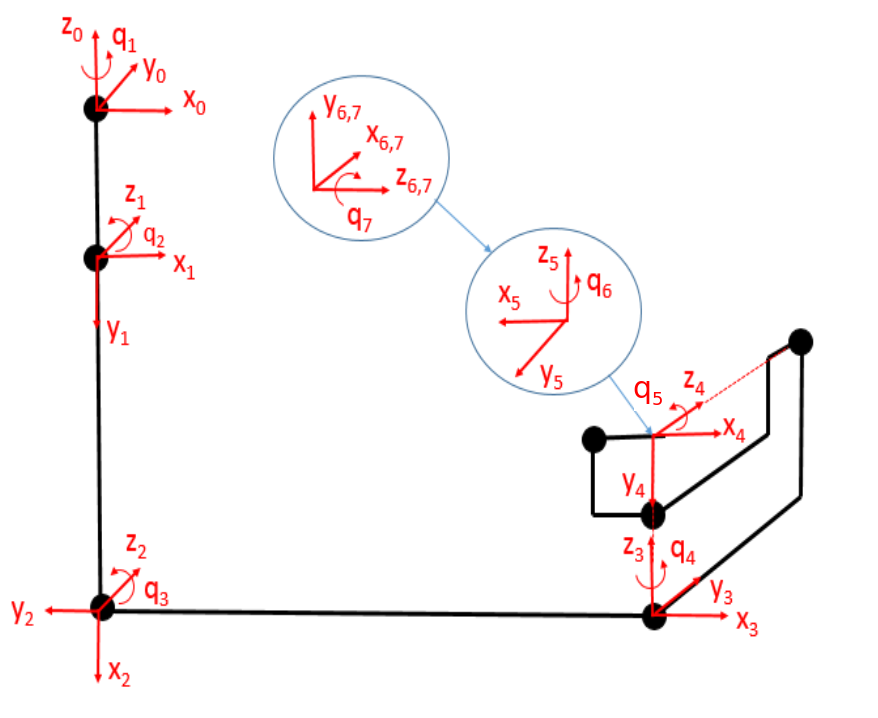
\includegraphics[width=3.0in]{dh_parameters}
\caption{Frames assignment of master arm using DH parameters.}
\label{dh_parameters}
\end{figure}

The home position is the position at which all joint positions are zero. Because the existing software assigned the positive joint directions, the team ensured that the DH parameters accurately reflected that assignment. Additionally, the team used symbolic representation for all lengths. The length parameters were difficult to accurately measure and were thus included in the parameter identification task. Utilizing previous work, the team used a MATLAB function to obtain the 4 x 4 homogeneous transformation matrices for each frame with respect to the base frame from the DH parameters.

\subsection{Lagrangian}
The next step in determining the G matrix is to compute the Lagrangian of the system. The Lagrangian will be utilized in the Euler-Lagrange approach to forward dynamics of robot manipulators. The Lagrangian of a system is given as:


\begin{equation}
\label{lagrangian}
L = K - P
\end{equation}

where K is the kinetic energy of the system and P is the potential energy. Because gravity compensation only account for torques in a stationary system, the kinetic energy term can be eliminated.

\begin{equation}
\label{lagrangian2}
L = -P
\end{equation}

The potential due to gravity is given as

\begin{equation}
\label{potential}
P = g \sum_{i=1}^n m_i h_i
\end{equation}

where g is the acceleration due to gravity, n is the number of masses, m is the mass, and h is the distance along the axis of g between the mass and the origin of the base frame. The masses were left as symbolic parameters to be identified. The h terms were determined using the transformation matrices from the forward kinematics. The h terms are functions of the robots pose. 


\subsection{Euler-Lagrange Equation}
The Euler-Lagrange equation allows for the calculations of generalized forces (torques or forces) from the derivatives of the Lagrangian.

\begin{equation}
\label{euler_lagrange}
\tau = \frac{\mathrm{d}}{\mathrm{d}{t}}\frac{\partial L}{\partial \dot{q}} - \frac{\partial L}{\partial q}
\end{equation}

Once again, this can be simplified by identifying terms that go to zero for a stationary manipulator.

\begin{equation}
\label{euler_lagrange2}
\tau = - \frac{\partial L}{\partial q}
\end{equation}

Using equation \ref{lagrangian2} and \ref{euler_lagrange2}, the symbolic torque terms necessary for gravity compensation can be determined.

\subsection{Setup}
The setup consisted of da Vinci MTM connected to the controller boards which reads the data from the MTM and communicate it to a ROS terminal. This ROS terminal has previously been setup with most of the software framework for the da Vinci robot. This terminal was further connected through a wireless link to a terminal running MATLAB with Robotic System Toolbox (RST). RST allows the team to read and write to the ROS topics. 

\begin{figure}[!t]
\centering
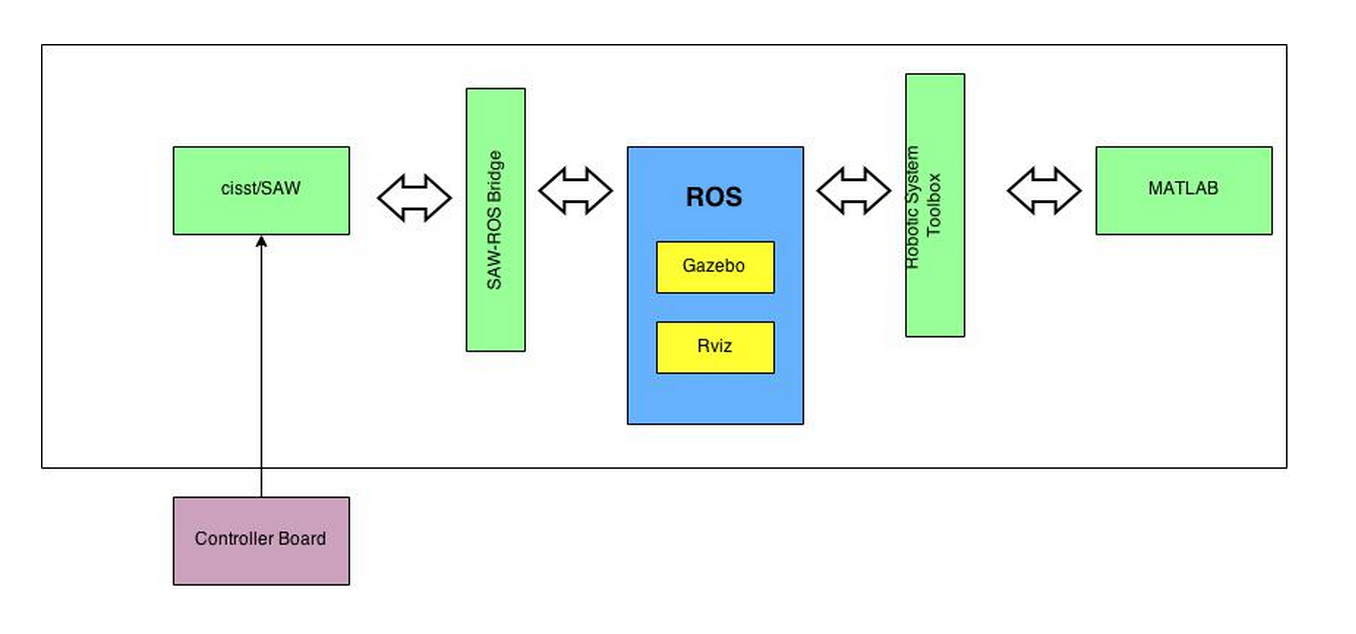
\includegraphics[width=3.25in]{setup}
\caption{Hardware \& Software Architecture of da Vinci Robot at WPI.}
\label{hardware_setup}
\end{figure}

\subsection{Data Collection Issues}
After developing the mathematical model the next step was to collect the corresponding torques and joint position data which will help us in estimating the parameters necessary for gravity compensation. As the team started with the task, several issues arose:


\begin{enumerate}

		\item\textit{ Communication issues } \\ The first issue that the team faced was that whenever a wireless device (like a laptop) was involved in the communication between ROS and the MATLAB RST terminal there were communication issues that prevented the device recognition for both the terminals. The quick fix for this was to modify the operating system's hosts file (for Linux it is located under home/etc/hosts) by adding the ip address and device name of the computer to which the system is attempting to communicate.
        
        \item \textit{Unstandardized message (msg) types} \\ The next issue that the team confront was that the already establish ROS framework for the da Vinci utilized some non-standardized msg types which are not readable in MATLAB. e.g. The Torque data had the msg type cisst/vecDoublev which MATLAB was not able to read. To solve this issue, the team implemented a ROS node that was able to create a new standardized topic type, read data from the unstandardized topic type and copy it to the new topic. This new topic was then read in MATLAB.

		\item \textit{Workspace restriction }\\ Another issue was that the operating space for the MTM was restricted by the frame of the robot in the laboratory. Consequently, the team was unable to operate the arm over the full range of its joints. If attempted, the arm would have crashed into the frame and potentially damaged the robot. This forced the team to work within the restricted workspace.
        
        \item \textit{Non-definitive joint limits} \\ For some of the joints, the joint limits are dependent upon the state of the previous joints. e.g. the limit of joint 3 was dependent upon the state of joint 2 . This caused the team to not have numerically constant hard limits for some of the joints. The team was able avoid the joint limits by the chosen method of collecting data.

\end{enumerate}


\subsection{Data Collection Strategy}
Our data collection strategy was designed so that we could get position and corresponding torque data at varying range of arm configurations and avoid all joint limits. The strategy was as follows:

\begin{enumerate}
		\item Place the MTM in a random pose by hand.
        \item Record the joint positions for each pose in MATLAB.
        \item Repeat steps 1 and 2 for desired number of poses
        \item Command the arm (from MATLAB) to move to recorded pose 
        \item Record the torque values necessary to hold the pose
        \item Repeat steps 4 and 5 for all recorded poses
\end{enumerate}

    
By following the above method, the team was able to get many data sets for torque and joint position values.

\subsection{Regressor and Parameter Matrices}
The next step was to divide our torque equations into a matrix of knowns (called the Regressor Matrix Y) and the matrix of the unknowns (called the Parameter matrix $\pi$). The parameter matrix consisted of products of unknown link lengths, link masses and locations of center of masses. After splitting, the team got a 7x12 Regressor Matrix and 12x1 parameter matrix.

\begin{equation}
\label{regression}
\tau = Y(q,\dot{q},\ddot{q})\pi
\end{equation}

\subsection{Least Square Method}
Now the team substituted each of our data sets into torque values and the regressor matrix. Then the team stacked these matrices on top of each other to form an equation  as shown below

\begin{equation}
\label{least_square}
\bar{\tau} = \begin{bmatrix}
       \tau(t_1)\\[0.3em]
       \vdots\\[0.3em]
       \tau(t_N)
     \end{bmatrix}
     		= \begin{bmatrix}
       Y(t_1)\\[0.3em]
       \vdots\\[0.3em]
       Y(t_N)
     \end{bmatrix} \pi = \bar{Y} \pi
\end{equation}

From this equation, the team calculated the estimates of the parameters by doing the left pseudo inverse of our ‘stacked regressor matrix’

\begin{equation}
\label{pseudo_inverse}
\pi = (\bar{Y}^T\bar{Y})^{-1}\bar{Y}\bar{\tau}
\end{equation}

Now that the team had the estimates of parameters, the team could get an estimate of the torques required for gravity compensation at some pose by substituting the joint position values into the regressor matrix and multiplying it with the estimates of parameter matrix.

\begin{figure}[!b]
\centering
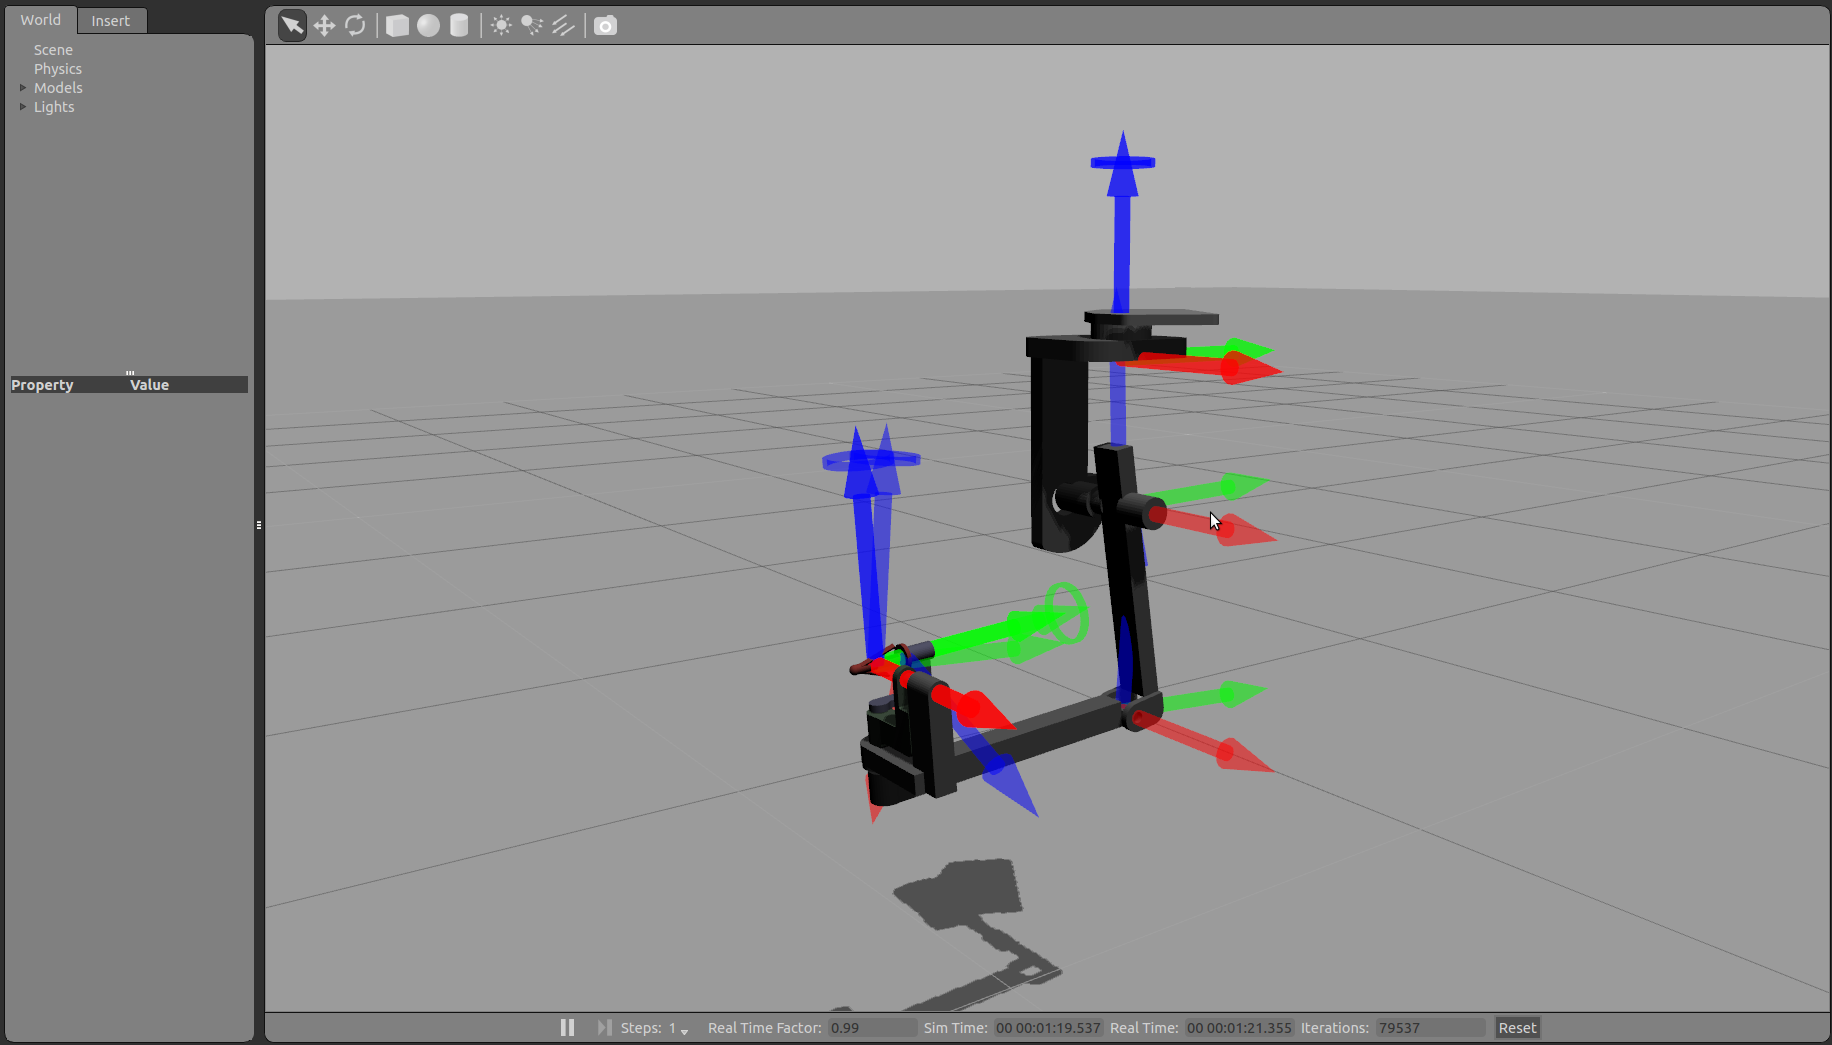
\includegraphics[width=3.25in]{mtm_joint}
\caption{MTM arm simulated in Gazebo with all active joints shown.}
\label{mtm_joint}
\end{figure}

\subsection{Modeling \& Simulation}
The gravity compensation control of da Vinci MTM arm was simulated using the Gazebo simulator by Open Source Robotics Foundation (OSRF) \cite{5}, as shown in Fig.~\ref{mtm_joint}. Gazebo has the capability to allow users to control each joint of the simulated robot through its internal controller. However, the team would be using the ros{\_}control package instead since it will allow us to use our own developed controller. Implementation of ros{\_}control package in Gazebo requires two main steps. The steps will be briefly described here, for more detail information refer to the ros control tutorial on Gazebo web page. The first step was to add the transmission elements into the Universal Robot Description Format (URDF) file of MTM. The transmission elements were responsible for actuating our robot joints. Joint name, type of transmission, and hardware interface need to be specified.  The second step was to include gazebo{\_}ros{\_}control plugin into our URDF model as well \cite{6}.

Once the plugin has been included, the team then proceeded to create the gravity compensation controller package. Many details will be omitted here for the sake of conciseness, refer to the Gazebo tutorial page for additional details. A ROS python node was created for our gravity compensation control implementation. This node subscribed to the joint{\_}state topic, calculated the required torque values for each joint based on the gravity compensation model and PID feedback, and finally published the torque commands to the joint(n){\_}controller/command topics. Furthermore, the desired joint configuration is also specified in this controller node, for this simulation we set zero radian for all joints as the desired configuration.

The PID feedback term was necessary since there was no a way, while simulating the torque control, to specify a position or hold the arm as done for the real robot. The control law is then given as:

\begin{equation}
\label{gravity_pid}
\tau = G(q_m) + K_p(q_d - q_m) + K_v(\dot{q}_d - \dot{q}_m) + K_i \sum (q_d - q_m)
\end{equation}

where $q_d$ = q desired and $q_m$ = q measured. Due to the way we defined the position and velocity error as $(q_d - q_m)$ and  $(\dot{q}_d - \dot{q}_m)$ respectively, $K_p, K_i$, and $K_v$ are positive definite. Furthermore, since we have seven joints to control, $K_p, K_i$, and $K_d$ are 7x7 diagonal matrices. The $G(q_m)$ vector was derived from the forward kinematic and center of mass locations specified in the MTM’s URDF file. The derivation would be similar to what was done for the real MTM. For the simulation, instead of estimating the parameters, the team used the parameters specified in the URDF file. For simplicity, all the masses are specified to be point masses and located at the joints. In the future, this parameter specifications can be updated with the estimated parameters found experimentally to improve the simulation model. Note that our work in this paper did not include all the estimated dynamics parameters. In the end, the team would obtain the gravity vector G(q) as a function of joint variables for our torque input.

The PID gains for the feedback term were tuned by first setting the $K_v$ and $K_i$ gains to be zero and adjusting the $K_p$ gains until the system produced constant amplitude oscillation. We then slowly increased the $K_v$ gains to damp the oscillation and finally increased the $K_i$ to correct for any steady state offset. Without the feed forward gravity term, normally this PID gains would have large gains. In this case, since the PID loop is only used to correct for the model error, the gains were relatively small.

In this paper we will also present our work on building the Gazebo model of patient side manipulator (PSM) arm. This work involved creating the model using the Simulator Description Format (SDF) because URDF does not currently support joint loops (parallel linkages) which is the case for the PSM arm. The virtual and collision elements are specified using the mesh files of PSM arm found in jhu dvrk github repository. SDF format requires users to specify the poses of all the links and joints of the robot. The poses for each link and joint are obtained by assembling the PSM CAD model in SolidWorks first and then using the measure feature to obtain the origin of each link with respect to the reference frame which in this case is the origin of the psm{\_}base{\_}link.

\section{RESULTS}
\subsection{Implementation on Real Robot}
The team determined numerical values for all twelve symbolic parameters determined using the symbolic torque equations. Using these values, the team wrote a MATLAB code that applied gravity compensation for a given position. Only gravity compensation terms were included in the applied torque, without any error based controller. At a rate of roughly one millisecond, the code read the joint positions and applied an appropriate torque. The visual results can be seen in the video results of this project.

The errors between the torque values read at positions and the torque values calculated using the determined parameters is shown in Fig.~\ref{result11} for joints 2 through 7. Joint 1 had a constant torque of zero when applying gravity compensation.

\begin{figure}[!t]
\centering
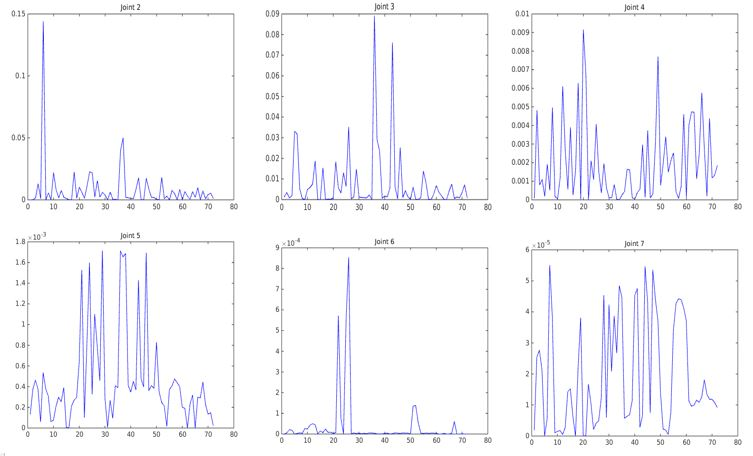
\includegraphics[width=3.25in]{Joint_Errors}
\caption{Square of joint error.}
\label{result11}
\end{figure}

\begin{figure}[!t]
\centering
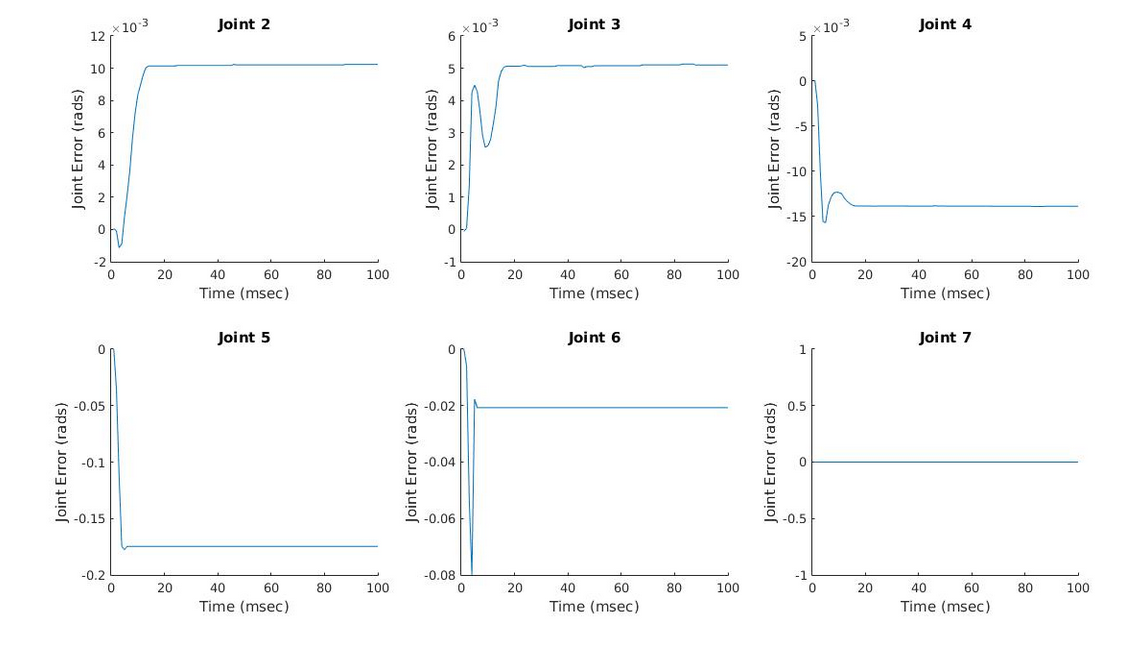
\includegraphics[width=3.25in]{result1}
\caption{Joint drift.}
\label{result12}
\end{figure}


Additionally, the team measured errors in joint values after the manipulator was realized when gravity compensation was being applied Fig.~\ref{result12}. As can be seen, the joint errors were less than 15 milliradians for joints 2 through 4. Joint 5 and 6 show greater errors and Joint 7 shows roughly 0 error.

\begin{figure}[!t]
\centering
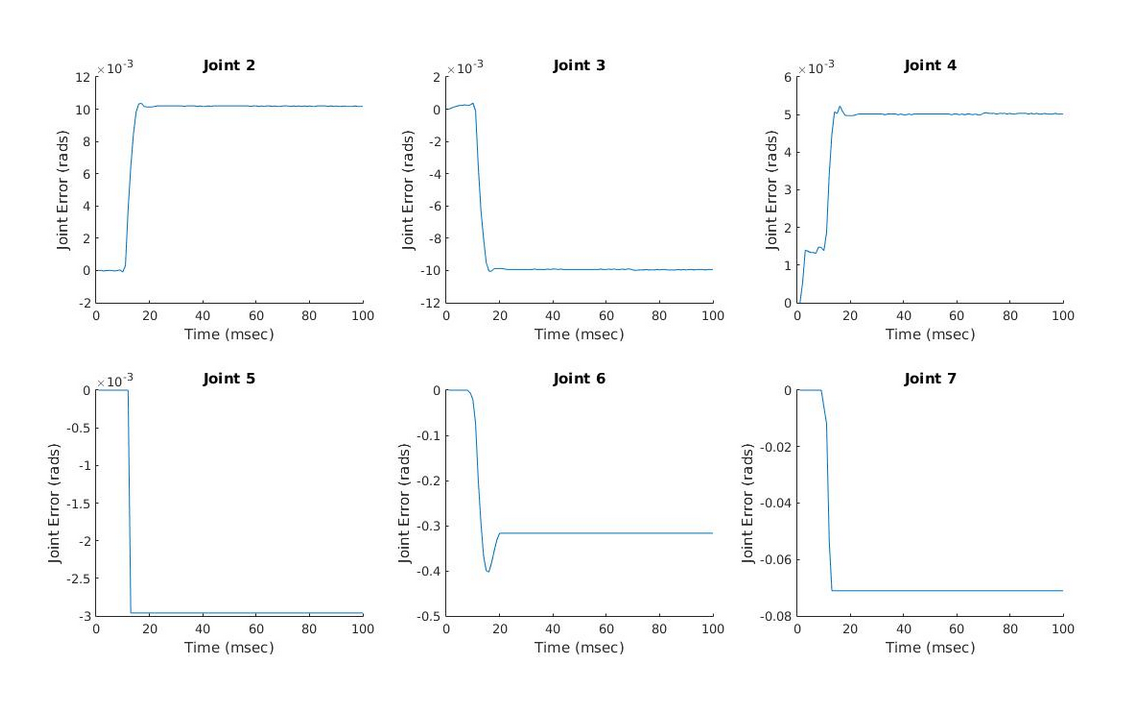
\includegraphics[width=3.25in]{result2}
\caption{Joint drift with some torques zeroed.}
\label{result2}
\end{figure}

While the team was satisfied that the arm maintained position using only the gravity compensation for most configurations, the orientation rarely held accurately. That is, joints 2 through 4 maintained positions while joints 5 through 7 did so rarely or at least inconsistently. Because of the low mass and length values for the last few links, the parameters were difficult to accurately determine. Regardless of the position when released, the joints 5 through 7 would move to a consistent position under gravity compensation. One solution to this issue is to set the torques for joints 5 through 7 to be zero during gravity compensation. This alleviates inaccurate torques which may be felt by an operator and allows for a small range of position to be held due to friction terms. The drift results for this condition can be seen in Fig.~\ref{result2}.


\subsection{Modeling and Simulation}

\begin{figure}[!b]
\centering
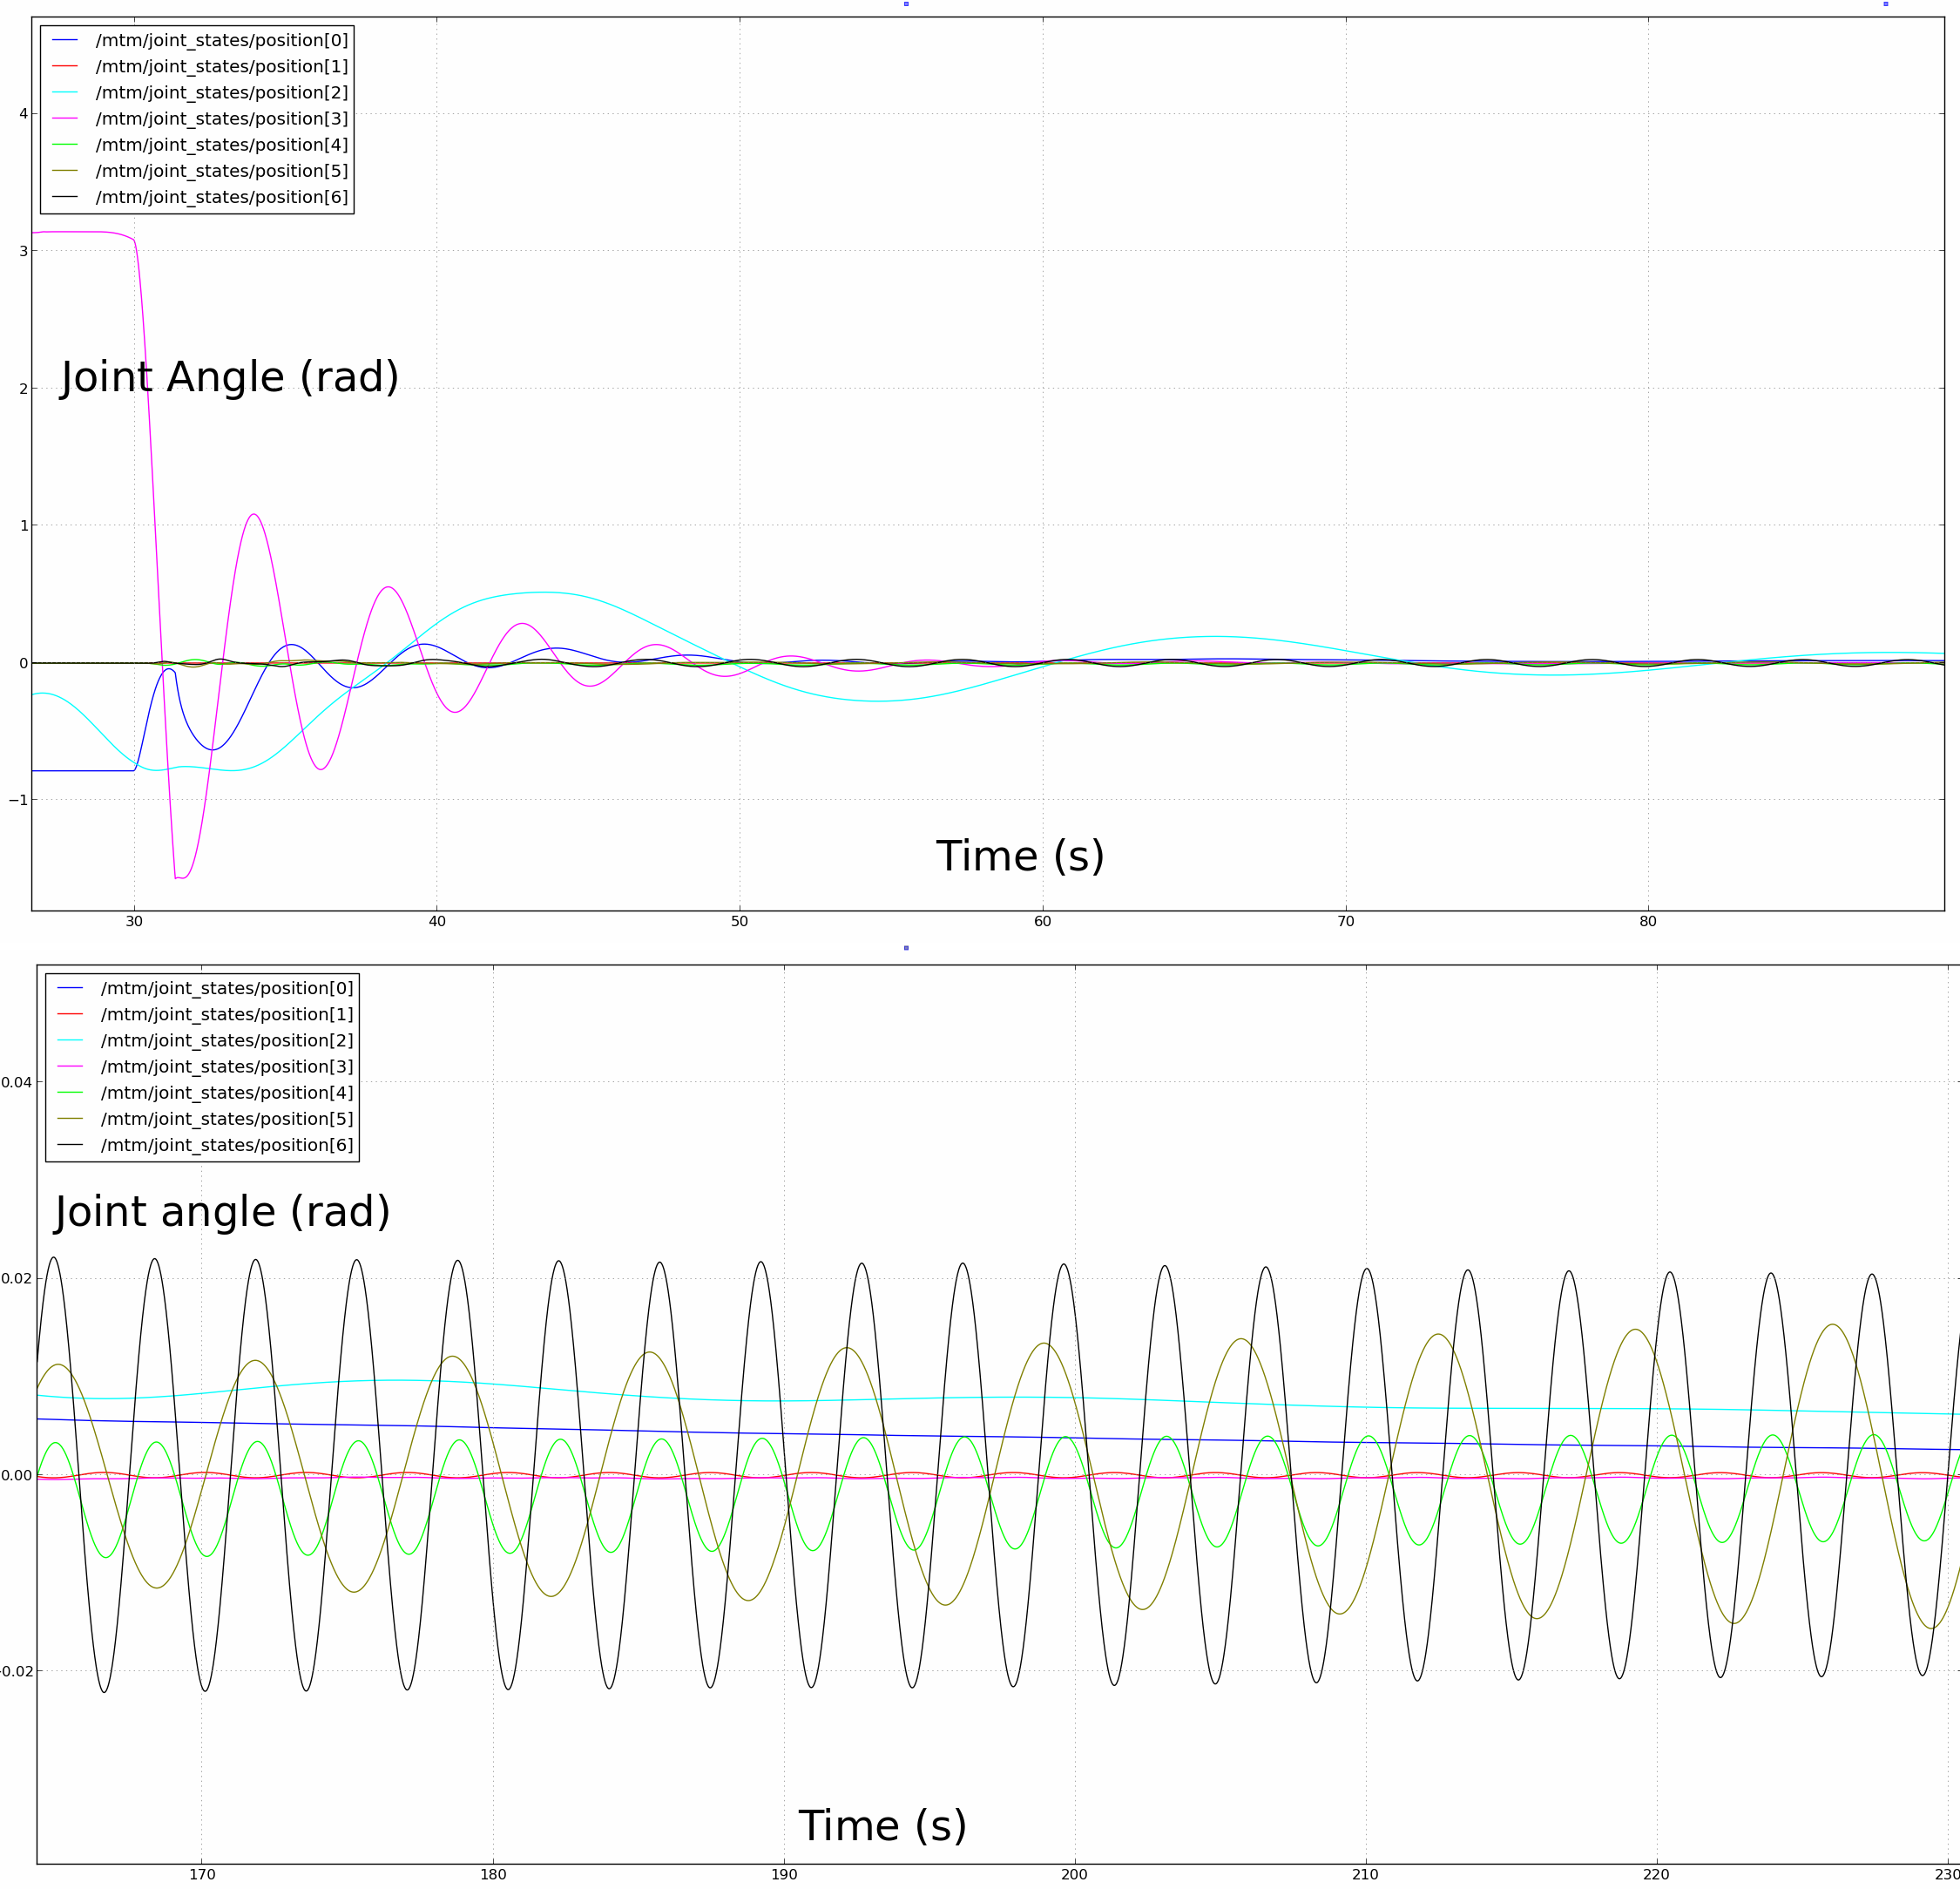
\includegraphics[width=3.25in]{mtm_result}
\caption{Joint angles as progression of time, top - wider view, bottom - close up view.}
\label{mtm_result}
\end{figure}

Fig.~\ref{mtm_result}  below shows the progression of the seven joint values as a desired position input of zero radians for all joints was applied. It appears that an underdamped response was present and all the joint values eventually seemed to converge to the desired value. However, upon a closer look of the system response as shown in Fig.~\ref{mtm_result}-bottom, the joint values did not exactly converge to zero, instead the values oscillated near zero. There is probably a need to better tune the gain values especially for the seventh joint, as the authors found it hard to keep this particular joint still. Nevertheless the team managed to obtain a stable system response.

\begin{figure}[!t]
\centering
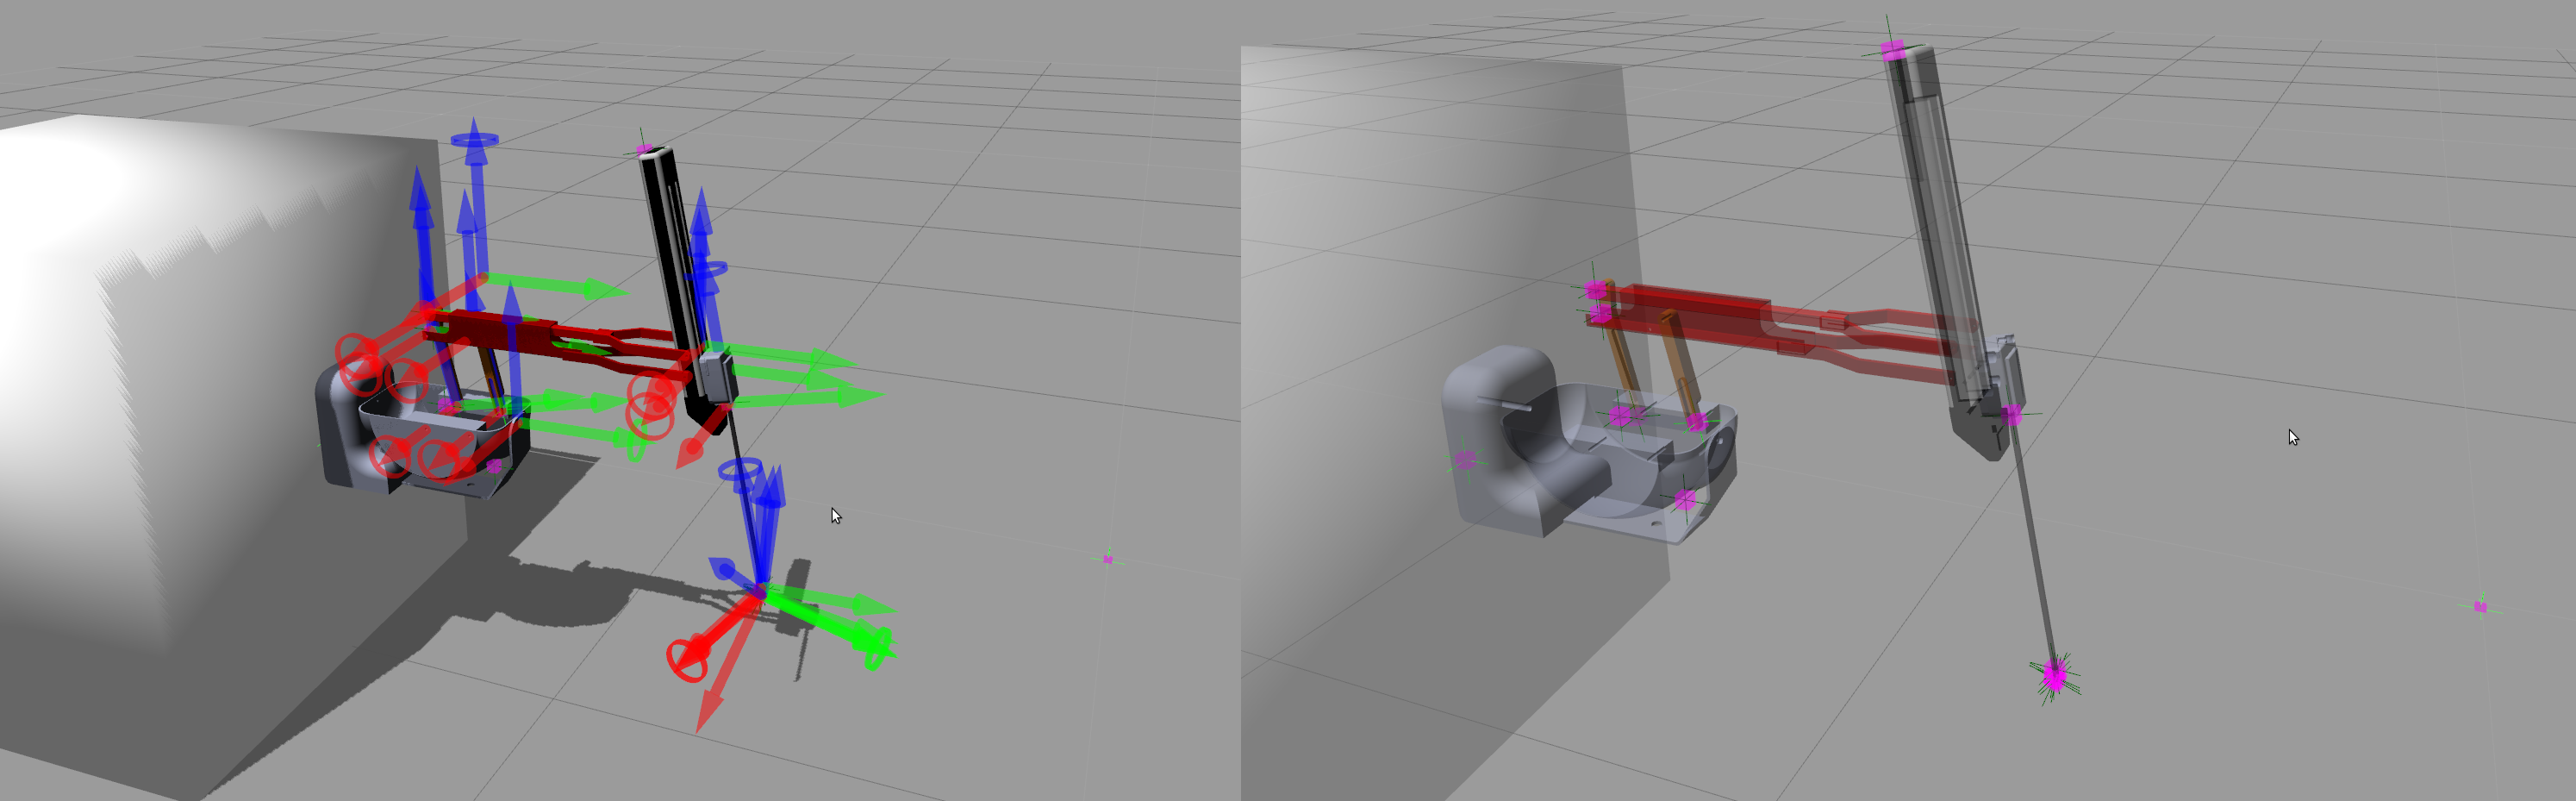
\includegraphics[width=3.25in]{psm_result}
\caption{left - PSM model with all joint locations shown, right - PSM model with center of mass locations.}
\label{psm_result}
\end{figure}

The PSM model described in the previous section is shown in Fig.~\ref{psm_result}. The PSM model contains seven revolute joints and one prismatic joint. Currently, all the center of masses are located at the joints for the sake of simplicity. In the future, the model can be improved by adjusting the center of mass locations with a result of a parameters estimation. All the joints of the PSM model can be torque controlled as was done for the MTM arm. This can be beneficial for future work done related to the PSM arm.


\section{CONCLUSION}
The team was successful in implementing gravity compensation on the main links of the MTM. Using the parameters derived from the least square fit, the arm was able to support itself with the correct gravity compensation. Similar gravity compensation was applied to the Gazebo model of the MTM, enabling it to be controlled as well. Finally, the team created a model of the PSM in Gazebo that could be used on similar projects in the future. Overall, the project has provided a very strong basis into allowing the operator full and accurate control over the da Vinci arm.


\begin{thebibliography}{1}

\bibitem{1}
P. Kazanzides, Z. Chen, A. Deguet, G. S. Fischer, R. H. Taylor, S. P. DiMaio. \emph{An Open-Source Research Kit for the da Vinci® Surgical System}, 2014.

\bibitem{2}
Z. Z. G. S. F. Adnan Munawar, \emph{Implementation of a Motion Planning Framework for the daVinci}, in Hamlyn Symposium on Medical Robotics, London, UK, 2014.

\bibitem{3}
W. Jun, W. Jinsong, Y. Zheng, \emph{An overview of dynamic parameter identification of robots, Robotics and Computer-Integrated Manufacturing}, Volume 26, Issue 5, October 2010, Pages 414-419, ISSN 0736-5845, http://dx.doi.org/10.1016/j.rcim.2010.03.013.

\bibitem{4}
Ping-An Bao; Ping Jiang; Hui-Tang Chen, "A learning scheme for the parameter identification of robot dynamics," Industrial Technology, 1996. (ICIT '96), Proceedings of The IEEE International Conference on , vol., no., pp.651,655, 2-6 Dec 1996

\bibitem{5}
M. Spong, S. Hutchinson and M. Vidyasagar, \emph{Robot modeling and control}. Hoboken, NJ: John Wiley \& Sons, 2006.


\bibitem{6}
K. Nate and H. Andrew. \emph{Design and use paradigms for gazebo, an open-source multi-robot simulator}. In Proceedings of the 2004 IEEE/RSJ International Conference on Intelligent Robots and Systems (IROS 2004), volume 3, pages 2149–2154, Sept 2004.

\bibitem{7}
Barros, Taiser Tadeu Teixeira; Fetter Lages, Walter, \emph{A Mobile Manipulator Controller Implemented in the Robot Operating System}, ISR/Robotik 2014; 41st International Symposium on Robotics; Proceedings of , vol., no., pp.1,8, 2-3 June 2014.

\end{thebibliography}

\end{document}